Having a single ion in the trap while sweeping the frequency or power would be ideal to determine the saturation parameter, and thus the fraction of \ce{Be+} in the excited \ce{^2P3/2} state. But due to the size and depth of our ion trap, we cannot reliably load only one ion, nor can we guarantee there only being one ion. On top of that, the most common residual gasses in a vacuum chamber, \ce{H2O} and \ce{H2} both readily react with \ce{Be+} in the excited state limiting the available interrogation time. Instead of a continuous measurement, we analyze images of ion chains at various laser powers and find the fluorescence per ion to fit to a generalized form of the scatter rate ($\Gamma_d$):

\begin{align}
	\Gamma_d & = a \rho_{pp} \nonumber \\
	& = \frac{a}{2}\frac{s}{1+s+4(\delta/\Gamma)^2} \label{eq: fluor fit}
\end{align}

Where the parameter $a$ consists of all the efficiency parameters in equation \ref{eq: fluorescence efficiency}. To get the P-state fraction, \ce{Be+} ions are loaded into the trap and A-ramps are applied until a chain is formed and the laser detuning adjusted until we see maximum fluorescence on the camera, which coincides with a detuning of $\Gamma/2$. Then images of the ions are taken at various laser powers and run through a maximum filter algorithm to identify the locations of individual \ce{Be+} ions as seen in figure \ref{fig: ion image set}. The portion of the image not an ion is then averaged to obtain the background pixel value, which is then subtracted from each localized ion image. The pixel values over each localized ion is then summed to yield a total fluorescence value, which is then averaged for each image, as shown in figure \ref{fig: local ions}. By performing a least squares fit on the collected fluorescence per ion as a function of incident power, we find the generalized efficiency $a$, revealing the P-state fraction at each power in $\rho_{pp}$, shown in figure \ref{fig: p state curve}.

\begin{figure}[H]
	\centering
	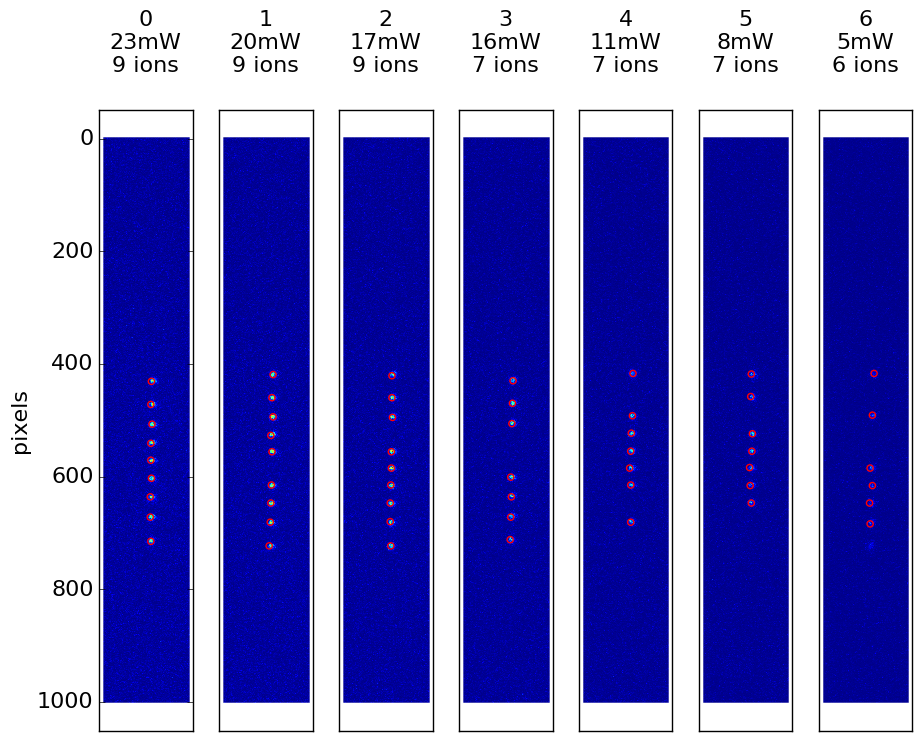
\includegraphics[width=0.8\textwidth]{images/ion_images.png}
	\caption{A set of ion images taken at various 313 nm powers run thorough a maximum filter algorithm that identifies local maxima, representing individual ions (circled in red). gaps in the ion chain are due to reactions with background \ce{H2} producing \ce{BeH+}, which occupy crystal sites without fluorescing.}
	\label{fig: ion image set}
\end{figure}

\newpage
\begin{figure}[H]
	\centering
	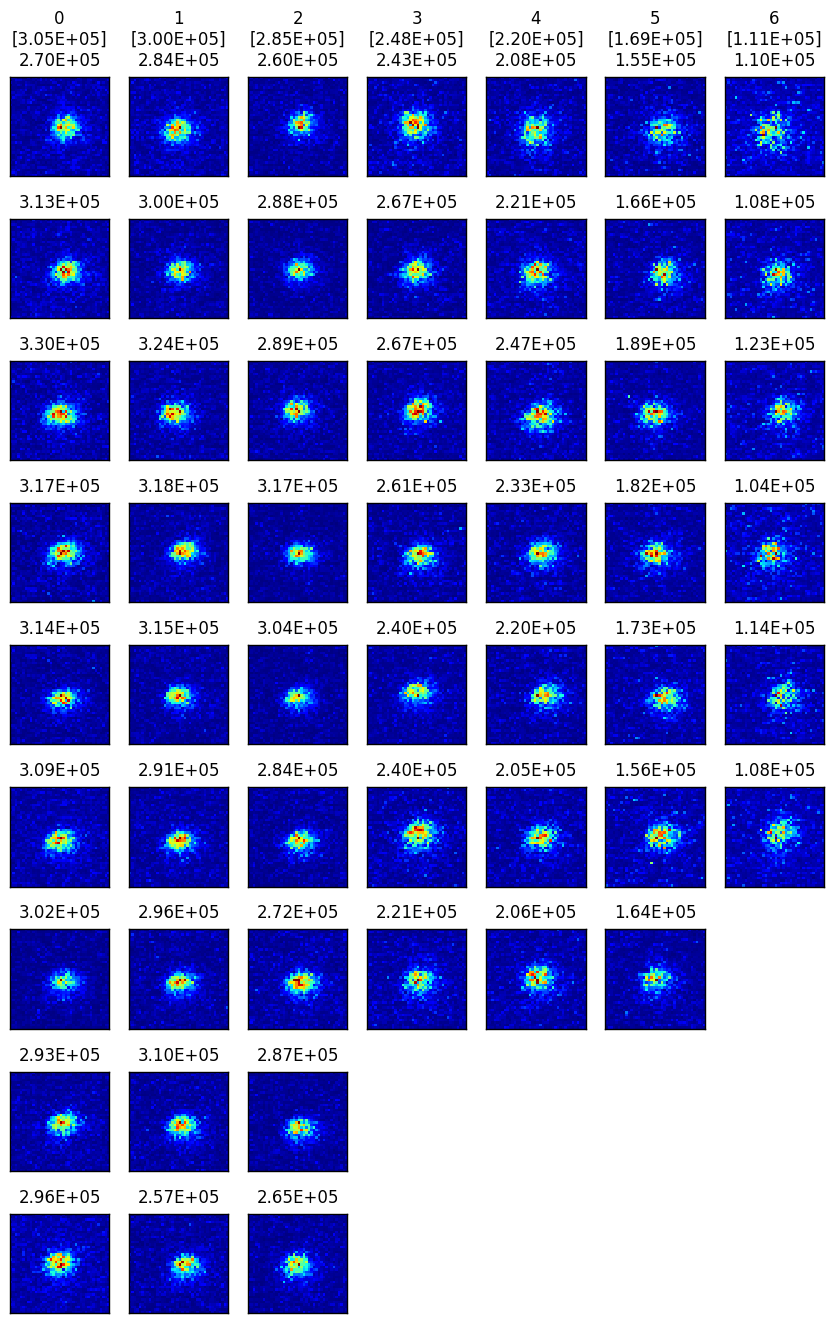
\includegraphics[height=0.7\paperheight]{images/isolated_ions.png}
	\caption{Individual ions identified from images in figure \ref{fig: ion image set}. Integrated pixel values with subtracted background counts shown for each image, a set's averaged value is shown in brackets.}
	\label{fig: local ions}
\end{figure}

\begin{figure}[H]
	\centering
	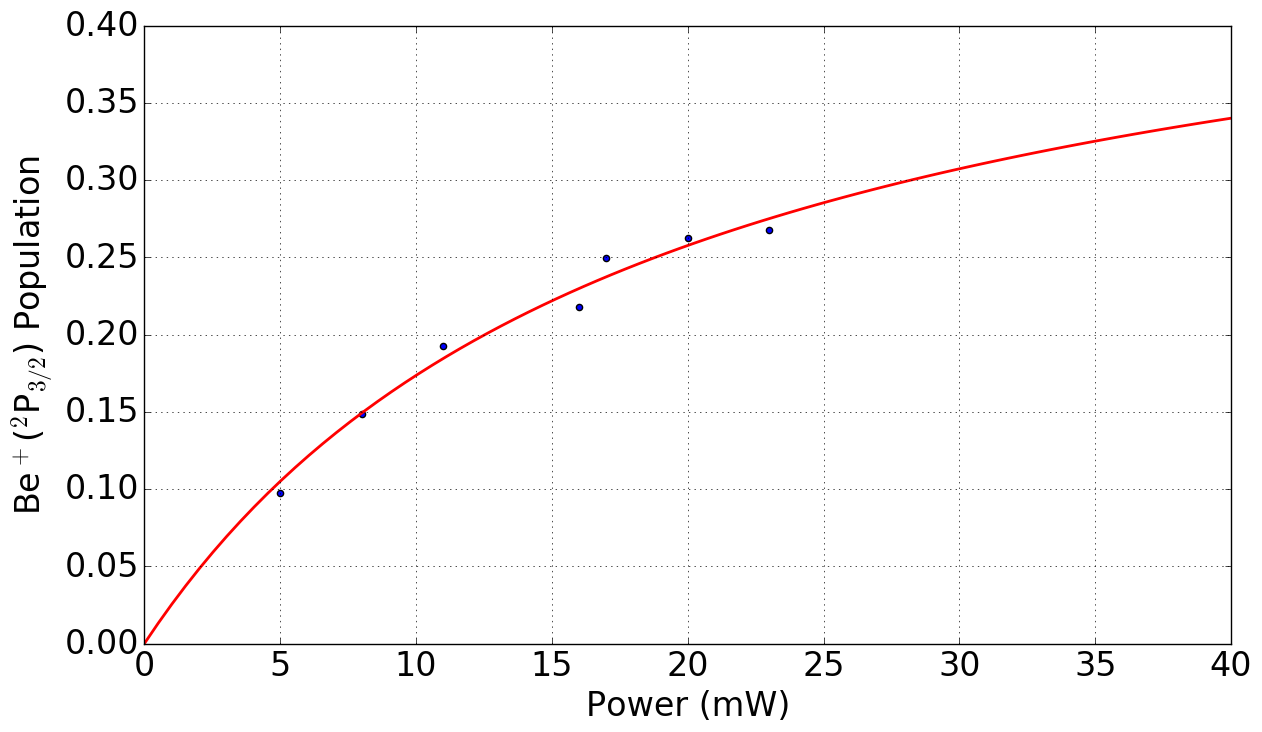
\includegraphics[width=0.8\textwidth]{images/P_state_curve.png}
	\caption{P-state fraction curve fitted to incident laser power at a fixed detuning of $\delta = \Gamma/2$. Total fluorescence value is normalized by fitted efficiency parameter $a$ to yield $\rho_{pp}$.}
	\label{fig: p state curve}
\end{figure}